
\section{Clock Skew Sensitivity}
\label{sec:results:csmb_sensitivity}

As explained in section~\ref{sec:methodology:sniper} one of the techniques that make Sniper faster than conventional cycle-accurate simulators, such as gem5, is the use of multiple simulation threads, each simulating one processor core.
In order to correctly simulate inter-core interactions, the simulation threads need to be kept in sync.
The method used to keep the threads in sync affects both simulation accuracy and simulation time.
By having a relaxed synchronization method, one can improve simulation time, at the cost of simulation accuracy.
In our experiments, we have used barrier synchronization with a barrier width of 100 cycles.
This entails that for every 100 simulated cycles the separate threads synchronize.
Any inter-core interactions that occur between two successive barriers are not guaranteed to happen in the correct order, but events separated by a barrier will be simulated in order.
In other words, within a single barrier there is the possibility that all simulation threads run sequentially.
For our work, this implies that there is a possibility that memory requests within a barrier arrives sorted by the core id, and not by time.
Because of this possibility we expect that changing the CSMB value could have a noticeable effect on our exprimentation results.

\begin{figure}
    \centering
    \begin{subfigure}[b]{0.5\textwidth}
        \includegraphics[width=\textwidth]{figures/results/speedup/csmb-stp-0128k-0100-csmb-4}
        \caption{STP sensitivity to CSMB}
        \label{fig:results:csmb:stp}
    \end{subfigure}%
    \begin{subfigure}[b]{0.5\textwidth}
        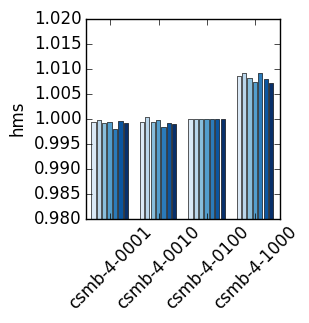
\includegraphics[width=\textwidth]{figures/results/speedup/csmb-hms-0128k-0100-csmb-4}
        \caption{HMS sensitivty to CSMB}
        \label{fig:results:csmb:hms}
    \end{subfigure}
    \begin{subfigure}[b]{0.6\textwidth}
        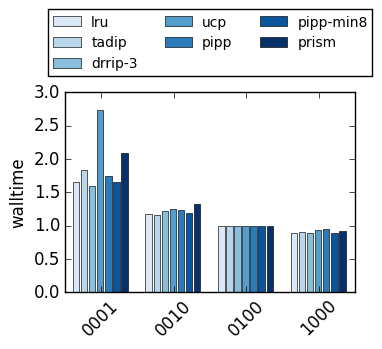
\includegraphics[width=\textwidth]{figures/results/speedup/csmb-walltime-0128k-0100-csmb-4}
        \caption{walltime sensitivity to CSMB}
        \label{fig:results:csmb:mpki}
    \end{subfigure}
    \caption{STP, HMS and walltime sensitivity to size of CSMB}
    \label{fig:results:csmb}
\end{figure}


We devised and experiment to investigate how much the choice of synchronization barrier width affects our results, and also how much it affects simulation time.
In the experiment, we vary the value of the clock skew minimization barrier (CSMB) and compare average STP, HMS and mpki values for all 4-core workloads.
Figure~\ref{fig:results:csmb} contains plots for both STP and HMS relative to the default 100 cycle barrier.
From the graph, it is apparent that lowering the value below 100 cycles causes negligible variations in our average values. 
The most noticeable is PIPP, that varies by only about 0.2\% with a tighter barrier interval.
Increasing the interval to 1000 cycles results in a more noticeable difference in measurements.
For both HMS, shown in figure~\ref{fig:results:csmb:hms}, and mpki, not shown, the trends are the same.

Variance in simulation time relative to CSMB values, as shown in figure~\ref{fig:results:csmb:walltime} is as expected. 
When lowering the barrier interval we measure an increase in average simulation time.
Increasing the barrier value causes a slight decrease in simulation time.
We observe that the performance gain by increasing the barrier is small compared to the result variation. 
Also when decreasing the barrier the result variation is small compared to the simulation time increase.
Based on this observation we find that 100 cycles is a good middle ground value for the synchronization barrier.

\todo{We could explain PIPP performance based on insertion position, and memory request serialization}
